\documentclass[a4paper,twoside, openright, 12pt, leqno]{article}
\usepackage[margin=0.5in]{geometry}
\usepackage{amsmath}
\usepackage{amsthm}                             % Proof environment
\usepackage{amssymb}
\usepackage{natbib}	
\usepackage{graphicx}
\usepackage{placeins}
\usepackage[document]{ragged2e}

% New command \xbar to make bar wider
\newcommand*\xbar[1]{%
   \hbox{%
     \vbox{%
       \hrule height 0.5pt % The actual bar
       \kern0.3ex%         % Distance between bar and symbol
       \hbox{%
         \kern-0.28em%      % Shortening on the left side
         \ensuremath{#1}%
         \kern-0.05em%      % Shortening on the right side
       }%
     }%
   }%
} 


\title{Revision to the paper ``The threshold age of the lifetable entropy''}


\date{\today}
% Hint: \title{what ever}, \author{who care} and \date{when ever} could stand 
% before or after the \begin{document} command 
% BUT the \maketitle command MUST come AFTER the \begin{document} command! 
\begin{document}

\maketitle

\section*{Editor}
\textbf{Both reviewers made a point of requesting more on why e0 and the threshold age are so similar. I would recommend that the authors respond to this comment. this response could be  (1) the addition of  some additional analysis explaining the connection, (2) the addition of  a footnote or a few sentences in the text explaining why the connection is not so clear and is a topic for future investigations, or (3) a response letter with the final manuscript explaining why you chose not to address this. I suspect that it is possible to show that in the case where mortality is Gompertz that the threshold very nearly approximates e0. The derivation probably can be done using the logic of Vaupel (1986), in which a/b is assumed to be negligible in size. Then, the empirical correspondence with e0 comes from the fact that mortality is roughly Gompertzian.}
\linebreak

We thank the editor for his suggestions. We have addressed reviewers' concerns assuming a Gompertz hazard, as suggested by the editor. We added further analysis and discussion on the connection between the threshold age and life expectancy based on the following:
\linebreak

Assume the force of mortality follows a Gompertz distribution with hazard $\mu(x) = \alpha\,\mathrm{e}^{\beta x}$, where $x\geq0$ denotes the age and $\alpha,\beta>0$ are parameters. The corresponding cumulative hazard is 
%%
$$
H(x)=\frac{\alpha}{\beta}\,\left(\mathrm{e}^{\beta x} - 1 \right).
$$
%%
Following \cite{wrycza2014entropy}, the lifetable entropy can be expressed in terms of the Gompertz parameters as
$$
\xbar{H}=\frac{1}{\beta}\,\left(\frac{1}{e_o}-\alpha\right)\;,
$$
%%
where $e_o$ is the life expectancy at birth. Plugging these two expressions into function $g(x)$ from Equation~(9) yields
\begin{equation}
g(x) = \frac{1}{\beta}\,\left(\alpha\,\mathrm{e}^{\beta x} - \frac{1}{e_o} \right)+\,\xbar{H}(x)-1\;.
\label{eq.gx}
\end{equation}

From Proposition~1 in the Appendix, the lifetable entropy conditioned on surviving to age $x$ can be expressed as
%%
$$
\xbar{H}(x)=\frac{e^\dagger(x)}{e(x)}=\frac{\int_x^\infty\,\ell(a)\,\big(H(a)-H(x)\big)\,da}{\int_x^\infty\ell(a)\,da}\;.
$$
%%
Using the above expressions in terms of the Gompertz parameters, it holds that the lifetable entropy conditional on surviving to age $x$ is
%
\begin{equation}
  \begin{split}
	\xbar{H}(x)
        & = \frac{\int_x^\infty \ell(a)\,\frac{\alpha}{\beta}\big(\mathrm{e}^{\beta a}-\mathrm{e}^{\beta x}\big)\,da}{\int_x^\infty\ell(a)\,da}=\frac{\int_x^\infty \ell(a)\,\alpha\,\mathrm{e}^{\beta a}\,da}{\beta\int_x^\infty\ell(a)\,da} - \frac{\alpha}{\beta}\,\mathrm{e}^{\beta x} 				\\
        & = \frac{\int_x^\infty\ell(a)\,\mu(a)\,da}{\beta\,e(x)\,\ell(x)} - \frac{\alpha}{\beta}\,\mathrm{e}^{\beta x}=\frac{1}{\beta}\left(\frac{1}{e(x)}-\alpha\,\mathrm{e}^{\beta x}\right)\;.
  \end{split}
  \label{eq.Hx}
\end{equation}
%
The last step in~\eqref{eq.Hx} uses the product $\ell(a)\,\mu(a)$ as the age-at-death distribution, which then implies that $\int_x^\infty \ell(a)\,\mu(a)\,da=\ell(x)$. Thus, $g(x)$ in~\eqref{eq.gx} reduces to

\begin{equation}
g(x) = \frac{1}{\beta}\,\left(\frac{1}{e(x)}-\frac{1}{e_o}\right)-1\;,
\label{eq.gx2}
\end{equation}
%
where $e(x)$ is the remaining life expectancy at age $x$. Equation~\eqref{eq.gx2} implies that the threshold age $a^H$ of the lifetable entropy $\,\xbar{H}$ under the Gompertz model occurs whenever
\begin{equation}
e(x) = \frac{e_o}{\beta\,e_o+1}\;.
\label{eq.threshold}
\end{equation}

Following \citet{missov2013gompertz}, the remaining life expectancy at age $x$ in the Gompertz case can be approximated by
%
\begin{equation}
  e(x)\approx\frac{1}{\beta}\,\mathrm{e}^{\alpha/\beta}\,\big(-\gamma-\ln(\alpha/\beta)-\beta x\big)\;,
  \label{eq:exapprox}
\end{equation}
%
where $\gamma\approx 0.57722$ is the Euler-Mascheroni constant. Hence, the threshold age occurs whenever
%
\begin{equation*}
\begin{split}
e(x)	& \approx\frac{1}{\beta}\,\mathrm{e}^{\alpha/\beta}\,\big(-\gamma-\ln(\alpha/\beta)-\beta x\big)=\frac{e_o}{\beta\,e_o+1}			\\
& \Longleftrightarrow x=-\frac{\mathrm{e}^{-\alpha/\beta}\,e_o}{\beta\,e_o+1}-\frac{1}{\beta}\,\big(\gamma+\ln(\alpha/\beta)\big)\;.
\end{split}
\end{equation*}

Note that from~\eqref{eq:exapprox}, $e_o\approx \mathrm{e}^{\alpha/\beta}\,\big(-\gamma-\ln(\alpha/\beta)\big)\,/\,\beta$. Using this approximation,
%
\begin{equation}
  \begin{split}
 	a^H & = -\frac{\mathrm{e}^{-\alpha/\beta}\,e_o}{\mathrm{e}^{\alpha/\beta}\,\left(-\gamma-\ln\left(\alpha\,/\,\beta\right)\right)+1}+\frac{e_o}{\mathrm{e}^{\alpha/\beta}}	\\
 	& = \frac{e_o}{\mathrm{e}^{\alpha/\beta}}\,\left(\frac{1}{\mathrm{e}^{\alpha/\beta}\,( \gamma+\ln\left(\alpha\,/\,\beta\right))-1}+1\right)	 \\
 	& = e_o\,\left(\frac{\gamma+\ln(\alpha/\beta)}{\mathrm{e}^{\alpha/\beta}\,( \gamma+\ln\left(\alpha\,/\,\beta\right))-1}\right)			 \\
 	& = e_o \cdot \delta\;,
  \end{split}
  \label{eq.x}
\end{equation}
%
which implies that the threshold age $a^H$ of the lifetable entropy $\,\xbar{H}$ for the Gompertz model is proportional to $e_o$ by a factor $\delta$ that only depends on $\alpha$, $\beta$ and $\gamma$. From equation~\eqref{eq.x}, the empirical correspondence between the threshold age and life expectancy at birth would come from $\delta$, which if it approximates one, it would  indicate that mortality in modern mortality schedules are roughly following a Gompertz model. Figure \ref{Fig:delta} shows the development of $\delta$ for French and Swedish females. The observation that this value converges towards one could be explanatory for the convergence of the threshold age and life expectancy at birth in modern mortality profiles. From this, it can be speculated that the difference between the threshold age and life expectancy in earlier years come from the fact that a big proportion of mortality was occurring in ages where the force of mortality does not follow a Gompertz such as in infancy.
\linebreak


\begin{figure}[h!]
\caption{Factor value $\delta$ for threshold age under Gompertz distribution for French and Swedish women.}
\centering
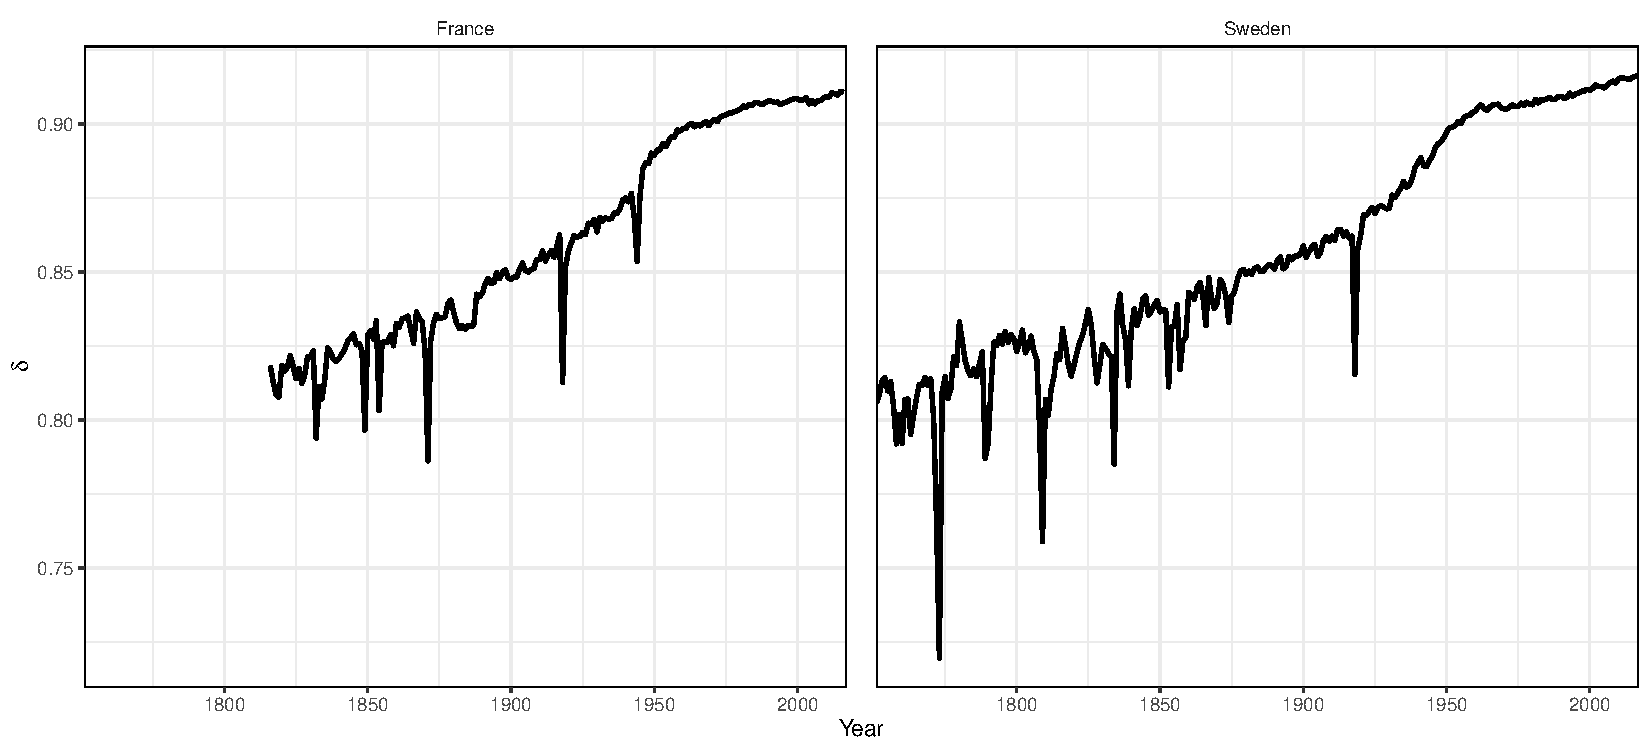
\includegraphics[scale=.5]{Figure_delta}
\label{Fig:delta}
\end{figure}

\FloatBarrier
%
%\noindent[VERSION 2: Lo que viene a continaucion es algo que he ido escribiendo en el proceso, aunque no lo pondria ya que creo que ha de primar la simplicidad. Pero como lo tengo hecho, pues por si lo quereis aprovechar]
%
%Following [ANYADIR Abramowitz and Stegun 1965??] \citet{missov2013gompertz} the remaining life expectancy at age $x$ in the Gompertz case is 
%%%
%$$
%e(x) = \frac{1}{\beta}\,e^{\alpha/\beta}\,E_1\left(\frac{\alpha}{\beta}\,e^{\beta x}\right),
%$$
%%%
%where $E_1(y)$ is the exponential integral 
%%%
%\begin{equation}
%  E_1(y) =\int_y^\infty\frac{e^{-t}}{t}\,dt=-\gamma-\ln(y)-\sum_{n=1}^\infty\frac{(-1)^n\, y^n}{n\cdot n!}\;, 
%  \label{eq:inteq}
%\end{equation}
%%%
%and $\gamma\approx 0.57722$ the Euler-Mascheroni constant. When $y=\alpha\,e^{\beta x}\,/\,\beta$ is close to 0, the summation on the right-hand side of~\eqref{eq:inteq} is negligible, and the remaining life expectancy of the Gompertz model can be approximated as
%$$
%  e(x)\approx\frac{1}{\beta}\,e^{\alpha/\beta}\,\left(-\gamma-\ln\left(\frac{\alpha}{\beta}\right)-\beta x\right)\;.
%$$
%
%Hence, the threshold age $a^H$ of the lifetable entropy $\,\xbar{H}$ under the Gompertz model occurs whenever
%%
%\begin{equation*}
%  \begin{split}
%	 e(x)	& \approx\frac{1}{\beta}\,e^{\alpha/\beta}\,\left(-\gamma-\ln\left(\frac{\alpha}{\beta}\right)-\beta x\right)=\frac{1}{\beta+1\,/\,e_o}			\\
%  	 & \Longleftrightarrow x=-\frac{e^{-\alpha/\beta}\,e_o}{\beta\,e_o+1}-\frac{1}{\beta}\left(\gamma+\ln\left(\frac{\alpha}{\beta}\right)\right)\;.
%  \end{split}
%\end{equation*}
%
%\noindent [END VERSION 2]
%\bigskip
%
%Then from \eqref{eq.threshold} the threshold age occurs when 
%%
%\begin{equation}
%\frac{1}{b} e^{a/b}\left[-\gamma - \ln\left(\frac{a}{b}\right) - bx - c \right] = \frac{1}{b+\frac{1}{e_o}},
%\label{eq.threshold2}
%\end{equation}
%%
%where $c = \sum_{n=1}^\infty \frac{(-1)^n (\frac{a}{b}e^bx)^n}{n \cdot n!}$ is the last term of the exponential integral. After some manipulation \eqref{eq.threshold2} yields
%
%%%
%$$
%-bx = e_o\left[ \frac{b}{e^{a/b}(e^{a/b}E_1(a/b)+1)} \right] + \gamma + \ln \left( \frac{a}{b} \right) + c.
%$$
%%%
%
%\noindent[PANCHO: Quiza me falla algo, pero aqui creo que no es correcto del todo: que C sea 0 no significa que $\gamma-\ln(a/b)$ lo sea]
%\bigskip
%
%To the extent that $c$ is close to 0, as suggested by \citet{missov2013gompertz}, then the threshold age $x$ from the above expression can be approximated by 
%%
%\begin{equation}
%  \begin{split}
%	x
%        & \approx e_o \left[\frac{1}{e^{a/b}}\left(1-\frac{1}{e^{a/b}(E_1(a/b)+1)} \right) \right] \\
%        & =  e_o \cdot \delta
%  \end{split}
%  \label{eq.x}
%\end{equation}
%%

\newpage
\textbf{Reviewer 1’s point: What insight does the threshold age for entropy give above and beyond the threshold age for e dagger? Why would we calculate one over the other? also seems worth addressing in order to improve the motivation of the paper and attract more readers.} \linebreak



All lifespan variation indicators are different in the way they are constructed and their formal properties. In this sense, if one is interested in measuring relative inequality, then the lifetable entropy is a better indicator than $e^\dagger$, which is an indicator of absolute inequality. Another advantage of the lifetable entropy is that it captures the dimensionless shape of aging \citep{colchero2016emergence}, which is desirable when comparing age-at-death distributions of different species, for example. If the lifetable entropy is used, the threshold age for $e^\dagger$ might be misleading regarding the effect of mortality changes, as we showed. This mismatch could lead to incorrect interpretation of some results. For example, in equation 10 in the manuscript, we are certain that if improvements happen at all ages, the early component is always negative (reducing the entropy) and the late component increases the entropy. This does not hold when the cut-off is derived with the threshold age of $e^\dagger$.


\section*{Reviewer A}
\textbf{Main Strengths:
Overall, this is a clearly laid out and interesting paper. The mathematical relationships are clearly specified and easy to follow.} \\

\textbf{Main Weaknesses:
My only suggestions are for a bit more of a detailed discussion around the insight that the threshold age provides and around Figures 1 and 2. In particular: What insight does the threshold age for entropy give above and beyond the threshold age for e dagger? Why would we calculate one over the other? }\linebreak


Lifetable entropy and $e^\dagger$ are both measures of lifespan variation, however, their demographic interpretation differs. The former one is defined as the elasticity of life expectancy due to changes in death rates \citep{keyfitz1968introduction} whereas the later one refers to the life expectancy (measured in years) lost due to death \citep{Vaupel1986}. Life table entropy is a measure of relative variability and $e^\dagger$ measures absolute lifespan variation. According to the framework developed by \citet{Wrycza2015}, lifetable entropy is preferred when comparing radically different distribution of deaths (i.e. distinct species across the tree of life). On the other hand, given its straight-forward interpretation (it is expressed in years), $e^\dagger$ has been used to obtain insights about lifespan variation among human sub-populations by social gradients (e.g. occupational class in \citet{vanRaalte2014} and income in \citet{bronnum2017socially}). Both measures are  meaningful and complementary. Depending on the aim of the study, the user should be able to select between measuring relative (lifetable entropy) or absolute ($e^\dagger$) variation. If the lifetable entropy is used, the threshold age for $e^\dagger$ might be misleading regarding the effect of mortality changes, as we showed. This mismatch could lead to incorrect interpretation of some results. For example, in equation 10 in the manuscript, we are certain that if improvements happen at all ages, the early component is always negative (reducing the entropy) and the late component increases the entropy. This does not hold when the cut-off is derived with the threshold age of $e^\dagger$.\linebreak


We added the following to the manuscript:
\linebreak

`` \textit{Even though the lifetable entropy and $e^\dagger$ are both measures of lifespan variation, their demographic interpretation differs. The former is defined as the elasticity of life expectancy due to changes in death rates \citep{keyfitz1968introduction} whereas the later one refers to the average years lost due to death \citep{Vaupel2011}. The life table entropy measures relative variability while $e^\dagger$ measures absolute lifespan variation. Therefore the lifetable entropy is appropriate to compare different shapes of age-at-death distributions across different species and over time \citep{baudisch2013pace,Wrycza2015}, while $e^\dagger$ has been used to obtain insights about lifespan variation in different countries and in sub-population groups (e.g. by occupational class or income \citep{vanRaalte2014,bronnum2017socially}). Both measures are meaningful and complementary but the calculation of their threshold ages should be performed accordingly to interpret correctly changes of age patterns of mortality.}''
\linebreak


\textbf{Looking at Figure 1, the natural question is “do we always expect the threshold age to be so close to e0?” Why or why not? Figure 2 somewhat answers this question with a “no” given the trends in historical periods, but this is not really discussed in the text. Why the convergence of the entropy threshold age and other measures (e0 and a dagger) over time? What is driving this? Given modern mortality conditions, do we always expect the threshold age to continue to be very close to life expectancy? Or is it possible it will diverge again with improvements at older ages?} 
\linebreak

Thanks for this observation. We addressed this observation following the Editor's suggestion (see answer to Editor above). In addition, we complemented that analysis with discussion on historical patterns of mortality. Indeed, since hunter-gathers to modern populations, death rates have decreased at all ages but mostly at young ages \citep{burger2012human}. These patterns are responsible for the rise of life expectancy at birth. In Sweden,  for example, $e_0$ trended upwards more rapidly during the period 1900-1950 (see Figure \ref{fig:Fig2}). Absolute lifespan variation ($e^\dagger$) and $\bar{H}$ reacted accordingly. The associated threshold ages react to this phenomenon in similar ways. The convergence of $e_0$ and $a^\dagger$ towards $a^H$ is consistent with these patterns and possibly explained by the fact that most mortality in modern mortality regimes is explained by the Gompertz model. These results are an exciting new venue for new research to fully understand the patterns that we observe.
\linebreak

We added the following paragraph:
\linebreak

\textit{Values for $a^\dagger$ are close to life expectancy throughout the period. However, around 1950 there is a crossover between $a^\dagger$ and $e_o$ such that $a^\dagger$ remained close to life expectancy but below it. This result shows that the threshold age $a^\dagger$ being below life expectancy is a modern feature of ageing populations with high life expectancy. From the beginning of the period of observation to the 1950s, the threshold age for the lifetable entropy was above life expectancy for both countries. During some periods $a^\dagger$ was roughly constant whereas life expectancy trended upwards. After the 1950s, $a^H$ converged towards life expectancy. We further analyzed this observation assuming the hazard follows a Gompertz model (see Appendix). Our analysis showed that the threshold age $a^H$ of the lifetable entropy $\,\xbar{H}$ for the Gompertz model is proportional to $e_o$ by a factor $\delta$ that depends on the Gompertz parameters. Moreover, this parameter $\delta$ indicates that the empirical correspondence between the threshold age and life expectancy at birth  comes from the fact that mortality in modern mortality schedules are roughly following a Gompertz model. Therefore, it can be speculated that the difference between the threshold age and life expectancy in earlier years come from the fact that a big proportion of mortality was occurring in ages where the force of mortality does not follow a Gompertz such as in infancy. This is consistent with historical patterns which suggest that, since hunter-gathers to modern populations, death rates have decreased at all ages but mostly at young ages \citep{burger2012human}. The code and data to reproduce these results are publicly available through the repository in the link...}

 
\FloatBarrier

\begin{figure}[h!]
	\centering
	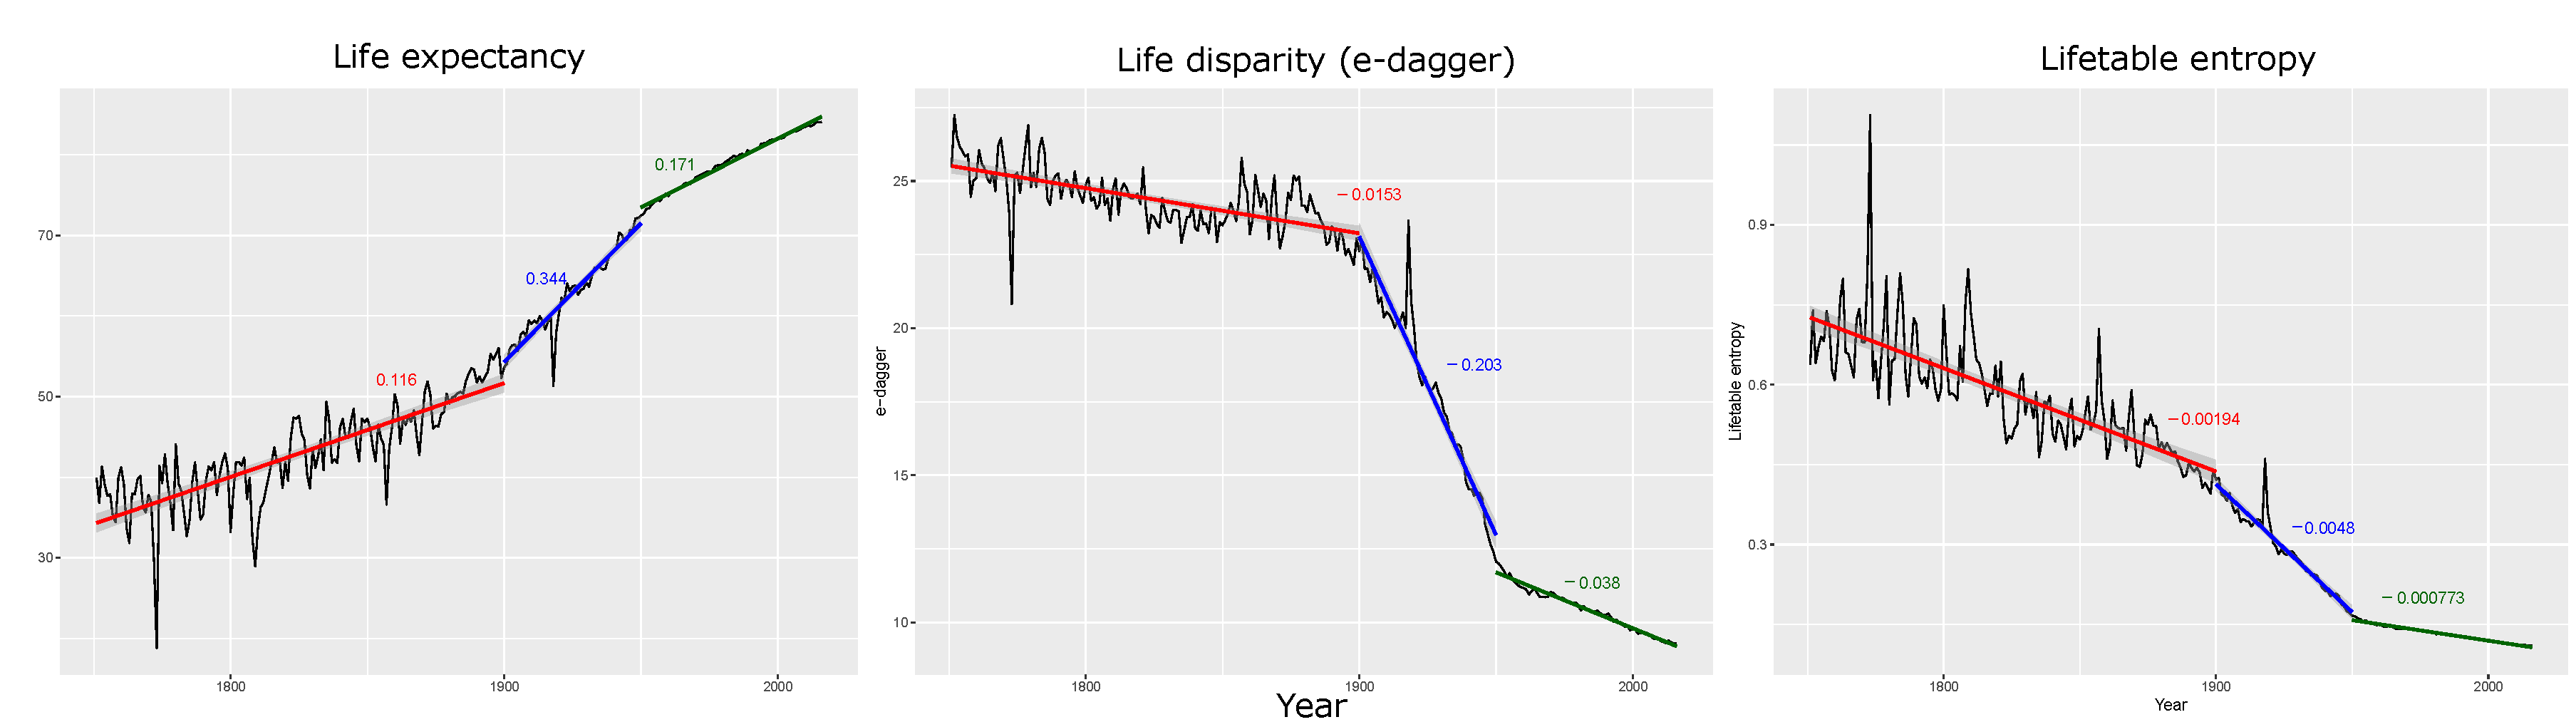
\includegraphics[scale=.31]{Figs_JA}
	\caption{Life expectancy at birth. $e^\dagger$ and lifetable entropy. Swedish females, 1750--2016. Source: \cite{HMD}}
	\label{fig:Fig2}
\end{figure}


\section*{Reviewer B}
\textbf{Main Strengths:
The paper presents interesting results related to an important measure for mortality studies, the Keyfitz entropy. The derivations are clear and provide useful and elegant results. These are certainly of interest to readers of the special collection on "Formal Relationships."}\\

\textbf{Main Weaknesses:
The point where the article could be improved is the "Applications" chapter. The authors could discuss in more details the interpretation of the threshold age for Keyfitz's, compared to e0 and the threshold age for e-dagger, as well as the implications of the findings of the paper for understanding mortality change and inequality of lifespans.} \textbf{Figure 2 presents intriguing results, but are not clearly interpreted in the paper. A few examples of topics that would be interest to discuss are: what are the features of mortality curve that make e0 and the threshold age for Keyfitz's entropy to converge?; and why were them so different for early years?; why is the threshold age for Keyfitz's entropy smoother than the other measures, even in periods of great mortality variation?}
\linebreak

We thank the reviewer for these suggestions and they were very similar to those mentioned by Editor and Reviewer A. As pointed out in the previous response to the Editor and Reviewer A, we approached in two different ways this suggestion. First we extended our analysis assuming the force of mortality follows a Gompertz model and from there we speculate on the convergence of the threshold age towards life expectancy. In addition, we extended the discussion on the lifetable entropy as indicator of lifespan variation.
\linebreak

\textbf{
Recommendations to Author:
In addition to the recommendation to expanding the interpretation of the results, there are a few minor suggestions:\\
On page 1, line 7, l(a) and l(x) are missing the t index.\\
On page 1, line 14, complement the sentence “remaining life expectancy at age a” with “at time t”.\\
On page 9, there is a typo in “Not the similarity”. \\
Review the last sentence of the conclusion, item (2). It doesn’t explain precisely what the threshold is about.}
\linebreak

We thank the reviewer for the careful read of our paper. Following her/his advice we have made all the changes suggested.

\bibliographystyle{dinat}
\bibliography{Bib_FormalDemo}

\end{document}
